%\clearpage


\begin{figure}[H]
\centering
\includegraphics[width=0.8\textwidth]{phase1_41.tikz}
\caption{Phase diagram packing density $\eta$ vs shell potential $\epsilon$ at constant $\lambda=1.4142$} \label{fig:phase_1_41}
\end{figure}

\subsubsection{The 1.4142 shell-to-core ratio}

Several studies\cite{dotera2014mosaic,stability} reported the existence of 2D quasi-periodic structures for the shell-to-core ratio of $\sqrt{2}$ %as well as the results from the section \ref{secqc1} where QC was found for close to 1.41 value 
which was a motivation to explore the $\sqrt{2}$ shell-to-core ratio in greater detail for 3D simulations.

Five phases were identified for the considered in the study $\eta-\epsilon$ range for $\lambda=1.4142$ -- disordered liquid, FCC/HCP with neighbor distance equal core radius,  QC, and two transition phases. No ordered structure was observed in the 0.25--0.50 packing density range. Hence the range is not included into the obtained $\eta-\epsilon$ phase diagram which is shown in the \textbf{Figure}  \ref{fig:phase_1_41}. % Another periodic structure was observed at 

\begin{figure}
\centering
%%%%%%%%% RDF
%FCC
\begin{subfigure}{.24\textwidth}
  \centering
  \includegraphics[width=0.97\textwidth]{r141s54e05.tikz}
  %\caption{}
  \label{fig:rdf141fcc} 
\end{subfigure}
% phase 1
\begin{subfigure}{.24\textwidth}
  \centering
  \includegraphics[width=0.97\textwidth]{r141s54e1.tikz}
  %\caption{}
  \label{fig:rdf14phase1} 
\end{subfigure}
% phase 2
\begin{subfigure}{.24\textwidth}
  \centering
  \includegraphics[width=0.97\textwidth]{r141s55e1.tikz}
  %\caption{}
  \label{fig:rdf14phase2} 
\end{subfigure}
% qc
\begin{subfigure}{.24\textwidth}
  \centering
  \includegraphics[width=0.97\textwidth]{r141s53e35.tikz}
  %\caption{}
  \label{fig:rdf14qc} 
\end{subfigure}
%%%%%%%%%%%%BOND
%FCC
\begin{subfigure}{.24\textwidth}
  \centering
   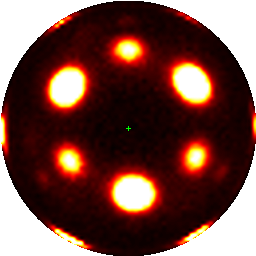
\includegraphics[width=0.67\textwidth]{l141s54e05}
  %\caption{}
  \label{fig:bond141fcc}  
\end{subfigure}
% phase 1
\begin{subfigure}{.24\textwidth}
  \centering
   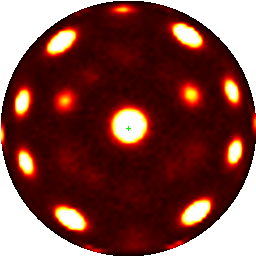
\includegraphics[width=0.67\textwidth]{l141s54e1}
 % \caption{}
  \label{fig:bond141phase1}  
\end{subfigure}
% phase 2
\begin{subfigure}{.24\textwidth}
  \centering
   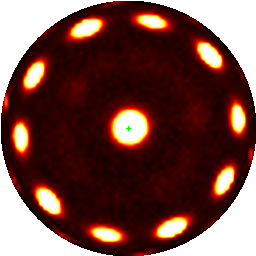
\includegraphics[width=0.67\textwidth]{l141s55e1}
  %\caption{}
  \label{fig:bond141phase2}  
\end{subfigure}
% qc
\begin{subfigure}{.24\textwidth}
  \centering
   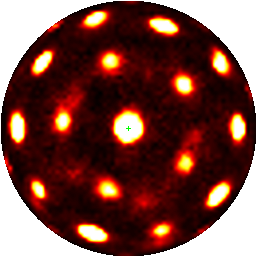
\includegraphics[width=0.67\textwidth]{l141s53e35}
  %\caption{}
  \label{fig:bond141qc}  
\end{subfigure}
%%%%%%%% Difff
%FCC
\begin{subfigure}{.24\textwidth}
  \centering
  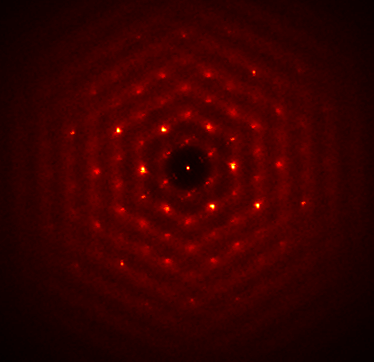
\includegraphics[width=0.95\textwidth]{dl141s54e05}
  \caption{}
  \label{fig:diff141fcc} 
\end{subfigure}
% phase 1
\begin{subfigure}{.24\textwidth}
  \centering
  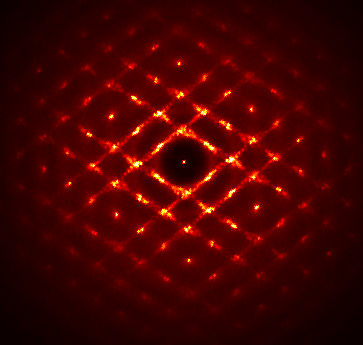
\includegraphics[width=0.95\textwidth]{dl141s54e1}
  \caption{}
  \label{fig:diff141phase1} 
\end{subfigure}
% phase 2
\begin{subfigure}{.24\textwidth}
  \centering
  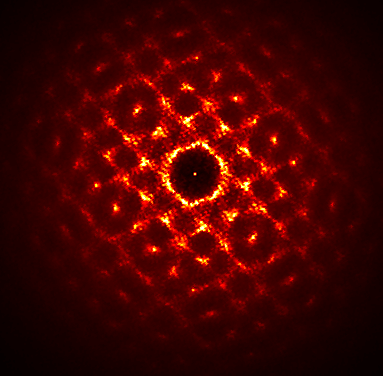
\includegraphics[width=0.95\textwidth]{dl141s55e1}
  \caption{}
  \label{fig:diff141phase2} 
\end{subfigure}
% qc
\begin{subfigure}{.24\textwidth}
  \centering
  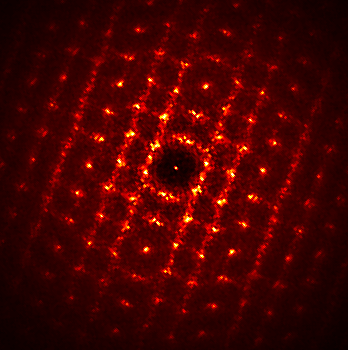
\includegraphics[width=0.95\textwidth]{dl141s53e35}
  \caption{}
  \label{fig:diff141qc} 
\end{subfigure}
\caption{Radial distribution functions, bond order diagrams and diffraction patterns of the structures, formed at  constant $\lambda=1.4142$. \subref{fig:diff141fcc} -- FCC/HCP structure, formed at $\eta=0.54$ and $\epsilon=0.5$, \subref{fig:diff141phase1} -- transition structure, formed at $\eta=0.54$ and $\epsilon=1.0$, \subref{fig:diff141phase2} -- another transition structure, formed at $\eta=0.55$ and $\epsilon=1.0$ and \subref{fig:diff141qc} -- QC structure, formed at $\eta=0.53$ and $\epsilon=3.5$}
\label{fig:evolution141}
\end{figure}

FCC/HCP structure forms at low values of shell potential. The increase in the shell potential forces particles to create transition structures. Two transition structures were recorded during my simulations. The first and the second structures, shown in the \textbf{Figures} \ref{fig:diff141phase1} and  \ref{fig:diff141phase2} respectively have a very similar to FCC/HCP RDF shape. The second structure apparently has a 10-fold symmetry. The formation of the transition structures is accompanied by the reduction of the 3rd peak on FCC/HCP RDF. In the final QC structure the 2nd, 3rd and 4th peaks on RDF have equal height. Basing on the RDFs from the \textbf{Figure} \ref{fig:evolution141} it can be concluded that the QC forms as a result of the particle rearrangement to a closer packed structure, hence the RDF 3rd peak located at about 1.9$R_{core}$ distance reduces its height, which apparently results in the 2nd peak at about 1.5$R_{core}$ distance growth. The moving particles change bond orientations, which is seen from the bond order diagrams. 


%QC structure appears when packing density approaches approximately 0.51. 
Stereographic projections of the bond order diagrams of the obtained QC structure together with the previously reported in the studies of %Engel et al.
\citet{methods} and %Damasceno et al.
\citet{compareicos} icosahedral QSs are shown in the \textbf{Figure} \ref{fig:stereocompare}. 
The shown in the \textbf{Figure} \ref{fig:myqc1} %and \ref{fig:qcfrominc} 
QC structure is similar to the \ref{fig:compare4}, however the RDF and the diffraction pattern appear to be different from previously published results. The QC phase is stable in a large range of varied parameters, however at high shell potential values the QC structure becomes very defective. 
%As seen from the figure the QC has different from the previously published results structure.

\begin{figure}
\centering
\begin{subfigure}{.19\textwidth}
  \centering
  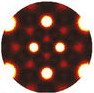
\includegraphics[width=0.97\textwidth]{compare1}
  \caption{}
  \label{fig:compare1} 
\end{subfigure}
\begin{subfigure}{.19\textwidth}
  \centering
   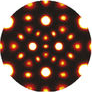
\includegraphics[width=0.97\textwidth]{compare2}
  \caption{}
  \label{fig:compare2}  
\end{subfigure}
%\begin{subfigure}{.19\textwidth}
 % \centering
 % \includegraphics[width=0.97\textwidth]{compare3}
 % \caption{}
 % \label{fig:compare3} 
%\end{subfigure}
\begin{subfigure}{.19\textwidth}
  \centering
  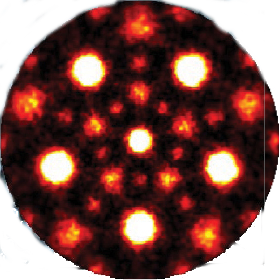
\includegraphics[width=0.97\textwidth]{compare4}
  \caption{}
  \label{fig:compare4} 
\end{subfigure}
\begin{subfigure}{.19\textwidth}
  \centering
   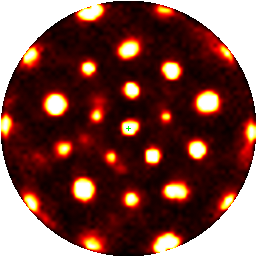
\includegraphics[width=0.97\textwidth]{s_0_53_e_3_50}
  \caption{}
  \label{fig:myqc1}  
\end{subfigure}
%\begin{subfigure}{.19\textwidth}
%  \centering
%   \includegraphics[width=0.97\textwidth]{sincrSters6l13}
%  \caption{}
%  \label{fig:qcfrominc}  
%\end{subfigure}
\caption{Comparison between bond order stereographic projections. Here \subref{fig:compare1}, \subref{fig:compare2} %, \subref{fig:compare3} 
and \subref{fig:compare4} are the projections of icosahedral QCs, obtained in the recent studies,\cite{methods, compareicos} %\subref{fig:myqc} and
\subref{fig:myqc1} %and \subref{fig:qcfrominc} 
--- the QC projection from this work for the parameters %$\lambda=1.4142$, $\eta=0.53$, $\epsilon=0.95$ and 
$\lambda=1.4142$, $\eta=0.53$, $\epsilon=3.5$ %and $\lambda=1.3$, $\eta=0.6$ from section \ref{secqc1} respectively
}
\label{fig:stereocompare}
\end{figure}

%Another observed in this work phase has the %similar to the hard sphere QC (\textbf{Figure} \ref{fig:rdf_psi}) 
%RDF shape, the bond oder diagram as well as the diffraction pattern , shown in the \textbf{Figure} \ref{fig:strangestructure}. 
%The phase probably represents a mixture of several phases.%, one of which is hard sphere .



% \begin{figure}
% \centering
% \begin{subfigure}{.3\textwidth}
%   \centering
%   \includegraphics[width=0.95\textwidth]{rdfstrange.tikz}
%   \caption{}
%   \label{fig:strangerdf} 
% \end{subfigure}
% \begin{subfigure}{.3\textwidth}
%   \centering
%    \includegraphics[width=0.95\textwidth]{s53E95}
%   \caption{}
%   \label{fig:strangebond}  
% \end{subfigure}
% \begin{subfigure}{.3\textwidth}
%   \centering
%   \includegraphics[width=0.95\textwidth]{Diffs53E95}
%   \caption{}
%   \label{fig:strangediff} 
% \end{subfigure}
% \caption{Radial distribution function, bond order diagram and diffraction pattern of the $\beta$ phase obtained at $\eta=0.53$, $\epsilon=1$ and constant $\lambda=1.4142$}
% \label{fig:strangestructure}
% \end{figure}


%The found QC has a unique structure, that does not seem to be previously reported elsewhere. 
%The diffraction patterns and bond order diagrams for various crystal orientations of obtained QC are provided in the \textbf{Figure} \ref{fig:qc2}. %The obtained QC phase seems to be not uniform. 
%Thus for high values of $\epsilon$ quasi-periodic phase is represented %mainly by 5-fold QCs, 
%by two phases while at lower values different quasi-periodic structure is observed. The obtained QC data is less noisy and for high $\epsilon$ values seems to resemble the results from the section \ref{secqc1} and thus a comparison with previously published data is possible. The \textbf{Figure} \ref{fig:stereocompare} shows four  previously observed in the works of Engel et al.\cite{methods} and Damasceno et al.\cite{compareicos} bond order stereographic projections (\textbf{Figures} \ref{fig:compare1}, \ref{fig:compare2}, \ref{fig:compare3} and \ref{fig:compare4}) of icosahedral QCs and %two QC projections 
%one QC projection from this work (\textbf{Figure} % \ref{fig:myqc} and 
%\ref{fig:myqc1}). As seen from the figure the 5-fold QC obtained in this work is different from to my knowledge all the previously published QC structures. The structure on the \textbf{Figure} %\ref{fig:myqc}
%is either same 5-fold QC with defects or another quasi-periodic phase.



% \begin{figure}
% \centering
% \begin{subfigure}{.24\textwidth}
%   \centering
%   \includegraphics[width=0.97\textwidth]{Bond_s_0_53_e_1_50}
%   %\caption{Bond order diagram}
%   \label{fig:qcbond2} 
% \end{subfigure}
% \begin{subfigure}{.24\textwidth}
%   \centering
%    \includegraphics[width=0.97\textwidth]{Diff_s_0_53_e_1_50}
%   %\caption{Diffraction pattern}
%   \label{fig:qcdif2}  
% \end{subfigure}
% \begin{subfigure}{.24\textwidth}
%   \centering
%   \includegraphics[width=0.97\textwidth]{Bond_s_0_53_e_1_50_6}
%   %\caption{Bond order diagram}
%   \label{fig:qcbond2_6} 
% \end{subfigure}
% \begin{subfigure}{.24\textwidth}
%   \centering
%    \includegraphics[width=0.97\textwidth]{Diff_s_0_53_e_1_50_6}
%   %\caption{Diffraction pattern}
%   \label{fig:qcdif2_6}  
% \end{subfigure}
% \caption{The bond order diagrams and diffraction patterns of the QC structure obtained at $\lambda=1.4142$, $\eta=0.53$ and $\epsilon=1.5$ for various crystal orientations}
% \label{fig:qc2}
% \end{figure}




%Thus Dotera et al.\cite{dotera2014mosaic} observed 12-fold QC for 
%The choice of shell-to-core ratio of $\sqrt[]{2}$ was motivated by recent reports of 2D quasi-periodic structures successful findings 